\scanpage{152}\mspage{7}%
A) Le formalisme des $Rf_!, f^!$ (combiné à $Rf_*, Lf^{\alpha}$, $\overset{\mathbb{L}}{\otimes}$ et $\mathbb{R}\mathrm{Hom}$, ``les six opérations'') porte implicitement en son sein la définition de l'homologie et l'identité essentielle entre fonctions homologiques et cohomologiques. \deleted{\unsure{E}} On dispose pour le moment de ce formalisme pour les faisceaux quasi-cohérents sur les schémas -- séminaire Hartshorne -- pour les espaces top. et les faisceaux de coeff. arbitraires dessus -- Verdier, exposé Bourbaki -- et en coh. étale des schémas pour les coefficients ``discrets'' \inserted{(de torsion ou ``$\ell$-adiques'')}%
% Local guide below the parenthetical insertion: the left end descends into
% the space after discrets and before premiers; there is no arrowhead.
\figure{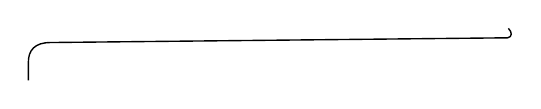
\begin{tikzpicture}[x=0.01cm,y=-0.01cm]
\draw[line width=0.5pt] (610,0) .. controls (615,5) and (615,11) .. (609,12)
 -- (28,18) .. controls (8,18) and (0,28) .. (0,43) -- (0,66);
\end{tikzpicture}}%
\uline{premiers aux \deleted{\unsure{le|la}} car. résiduelles} -- SGA 5 --%
% Local right guide, from the space after SGA 5 down towards the analytic
% insertion. The semicolon-shaped mark is inside the hook, above the
% Verdier--Ruget portion; its logical attachment is uncertain. It is not
% moved to a baseline before or after the inserted sentence.
\figure{\begin{tikzpicture}[x=0.015cm,y=-0.015cm]
\draw[line width=0.5pt] (90,0) .. controls (90,20) and (86,25) .. (62,27)
 -- (34,28) .. controls (12,28) and (5,43) .. (0,78);
\node[inner sep=0pt] at (22,58) {\unsure{;}};
\end{tikzpicture}}%
\inserted{enfin pour les faisc. coh. sur les espaces analytiques -- Verdier-Ruget --} (Le formalisme reste à développer dans le contexte cristallin, et en car. $0$ dans le contexte des modules stratifiés \inserted{à singularités}%
% Local guide below singularités, above à la. The isolated point at the
% left is below the early letters of stratifiés, not baseline punctuation.
% Source coordinates for both elements are recorded separately in report.json.
\figure{\begin{tikzpicture}[x=0.01cm,y=-0.01cm]
\path[use as bounding box] (0,65) rectangle (577,136);
\node[inner sep=0pt] at (88,113) {\unsure{.}};
\draw[line width=0.5pt] (363,127) .. controls (353,96) and (359,79) .. (401,75)
 .. controls (423,71) and (437,72) .. (448,76)
 .. controls (491,94) and (544,98) .. (567,94);
\end{tikzpicture}}%
à la Deligne, avec éventuellement -- sur le corps $\mathbb{C}$ -- des structures de Hodge à la clef, enfin dans le contexte des motifs ; je suis persuadé qu'il est présent un%
% Isolated short point below the initial u of un: uncertain intentional
% status, retained below its word rather than inserted into baseline prose.
\figure{\begin{tikzpicture}[x=0.01cm,y=-0.01cm]
\path[use as bounding box] (0,0) rectangle (80,45);
\node[inner sep=0pt] at (13,34) {\unsure{.}};
\end{tikzpicture}}%
peu partout encore -- partout, peut-être, où il y a un formalisme de nature cohomologique.) Travaillant en coh. étale sur un schéma \inserted{séparé}%
% Local guide below séparé, curving down into the space immediately before de.
\figure{\begin{tikzpicture}[x=0.015cm,y=-0.015cm]
\draw[line width=0.5pt] (94,0) .. controls (112,-5) and (113,8) .. (98,15)
 .. controls (77,25) and (48,29) .. (26,36)
 .. controls (2,43) and (-1,49) .. (0,61)
 .. controls (0,66) and (1,72) .. (4,76);
\end{tikzpicture}}%
de t.f. sur un corps $k$, disons, avec%
% Compact isolated point below the beginning of avec, above the final line.
\figure{\begin{tikzpicture}[x=0.01cm,y=-0.01cm]
\path[use as bounding box] (0,0) rectangle (105,45);
\node[inner sep=0pt] at (20,33) {\unsure{.}};
\end{tikzpicture}}%
un anneau de \unsure{coeff.|coeff} $\Lambda$ de \unsure{torsion} \unsure{premier} à \unsure{la} \unsure{car.|car}%
% The lower edge cuts this last line. No separate comma is recoverable after car.
% archive sheet number: 152
